\documentclass[conference]{IEEEtran}
\IEEEoverridecommandlockouts
% IEEEtran expects Times. pdfLaTeX gets it from the class; XeLaTeX/Tectonic
% has no Times in the TU encoding and would silently fall back to upright
% Latin Modern (no bold or italic), so load the TeX Gyre Times/Courier clones.
\usepackage{iftex}
\ifTUTeX
  \usepackage{fontspec}
  \setmainfont{texgyretermes}[Extension=.otf, UprightFont=*-regular,
    BoldFont=*-bold, ItalicFont=*-italic, BoldItalicFont=*-bolditalic]
  \setmonofont{texgyrecursor}[Extension=.otf, UprightFont=*-regular,
    BoldFont=*-bold, ItalicFont=*-italic, BoldItalicFont=*-bolditalic]
\fi
\usepackage{cite}
\usepackage{amsmath,amssymb}
\usepackage{graphicx}
\usepackage{booktabs}
\usepackage{xcolor}
\usepackage{url}
\usepackage{placeins}
\usepackage{tikz}
\usetikzlibrary{positioning}
\usepackage[hidelinks]{hyperref}
\newcommand{\sys}{\textsc{TailTag}}
\newcommand{\todo}[1]{\textcolor{red}{#1}}
\IfFileExists{generated/macros.tex}{\newcommand{\ovLossCpuNone}{0.0}
\newcommand{\ovCpuCpuNone}{0.0}
\newcommand{\ovNsCpuNone}{0}
\newcommand{\ovLossKvNone}{0.0}
\newcommand{\ovCpuKvNone}{0.0}
\newcommand{\ovNsKvNone}{0}
\newcommand{\ovLossCpuCount}{0.4}
\newcommand{\ovCpuCpuCount}{1.1}
\newcommand{\ovNsCpuCount}{411}
\newcommand{\ovLossKvCount}{-33.2}
\newcommand{\ovCpuKvCount}{1.2}
\newcommand{\ovNsKvCount}{98}
\newcommand{\ovLossCpuShm}{-2.7}
\newcommand{\ovCpuCpuShm}{0.6}
\newcommand{\ovNsCpuShm}{220}
\newcommand{\ovLossKvShm}{-29.1}
\newcommand{\ovCpuKvShm}{1.4}
\newcommand{\ovNsKvShm}{122}
\newcommand{\ovLossCpuAttrib}{2.4}
\newcommand{\ovCpuCpuAttrib}{27.5}
\newcommand{\ovNsCpuAttrib}{10431}
\newcommand{\ovLossKvAttrib}{9.6}
\newcommand{\ovCpuKvAttrib}{54.0}
\newcommand{\ovNsKvAttrib}{6405}
\newcommand{\ovLossCpuStream}{3.3}
\newcommand{\ovCpuCpuStream}{62.8}
\newcommand{\ovNsCpuStream}{22946}
\newcommand{\ovLossKvStream}{21.1}
\newcommand{\ovCpuKvStream}{53.1}
\newcommand{\ovNsKvStream}{7706}
\newcommand{\streamDropPct}{0.00}
\newcommand{\apAlFTest}{0.65}
\newcommand{\faAlFTest}{18104}
\newcommand{\apAlLTest}{0.55}
\newcommand{\faAlLTest}{29038}
\newcommand{\apAlFHeld}{0.42}
\newcommand{\faAlFHeld}{39248}
\newcommand{\apAlLHeld}{0.50}
\newcommand{\faAlLHeld}{32698}
\newcommand{\apAgFTest}{0.63}
\newcommand{\faAgFTest}{268629}
\newcommand{\apAgLTest}{0.58}
\newcommand{\faAgLTest}{394978}
\newcommand{\apAgFHeld}{0.24}
\newcommand{\faAgFHeld}{950128}
\newcommand{\apAgLHeld}{0.26}
\newcommand{\faAgLHeld}{16205}
\newcommand{\apQFTest}{0.94}
\newcommand{\faQFTest}{19618}
\newcommand{\apQLTest}{0.94}
\newcommand{\faQLTest}{19618}
\newcommand{\apQFHeld}{0.39}
\newcommand{\faQFHeld}{58371}
\newcommand{\apQLHeld}{0.55}
\newcommand{\faQLHeld}{58371}
\newcommand{\apQAlFTest}{0.96}
\newcommand{\faQAlFTest}{12187}
\newcommand{\apQAlLTest}{0.96}
\newcommand{\faQAlLTest}{21533}
\newcommand{\apQAlFHeld}{0.47}
\newcommand{\faQAlFHeld}{57555}
\newcommand{\apQAlLHeld}{0.60}
\newcommand{\faQAlLHeld}{60576}
\newcommand{\apQAgFTest}{0.96}
\newcommand{\faQAgFTest}{12236}
\newcommand{\apQAgLTest}{0.96}
\newcommand{\faQAgLTest}{16044}
\newcommand{\apQAgFHeld}{0.36}
\newcommand{\faQAgFHeld}{60890}
\newcommand{\apQAgLHeld}{0.57}
\newcommand{\faQAgLHeld}{57418}
\newcommand{\apRuleTest}{0.55}
\newcommand{\pRuleTest}{0.85}
\newcommand{\rRuleTest}{0.41}
\newcommand{\apRuleHeld}{0.53}
\newcommand{\pRuleHeld}{0.51}
\newcommand{\rRuleHeld}{0.67}
\newcommand{\apAggRuleTest}{0.45}
\newcommand{\apAggRuleHeld}{0.18}
\newcommand{\genOk}{73}
\newcommand{\genAll}{90}
\newcommand{\genMax}{24\,ms}
\newcommand{\noiseMed}{0.6}
\newcommand{\ruleTau}{0.04}
\newcommand{\valRuns}{115}
\newcommand{\valWithin}{97.8}
\newcommand{\valCoverage}{100.00}
\newcommand{\valDrops}{0}
\newcommand{\trainRuns}{54}
\newcommand{\testRuns}{36}
\newcommand{\heldRuns}{25}
\newcommand{\ewApTest}{0.95}
\newcommand{\ewPersTest}{0.82}
\newcommand{\ewBaseTest}{0.49}
\newcommand{\ewApHeld}{0.82}
\newcommand{\ewPersHeld}{0.62}
\newcommand{\ewBaseHeld}{0.28}
\newcommand{\sigCpuHogRunq}{284.8}
\newcommand{\sigCpuHogWake}{26.9}
\newcommand{\sigCpuHogIrq}{0.9}
\newcommand{\sigCpuHogBlk}{1.0}
\newcommand{\sigCpuFloodRunq}{3.1}
\newcommand{\sigCpuFloodWake}{0.7}
\newcommand{\sigCpuFloodIrq}{1.6}
\newcommand{\sigCpuFloodBlk}{1.0}
\newcommand{\sigCpuIoRunq}{1.0}
\newcommand{\sigCpuIoWake}{1.2}
\newcommand{\sigCpuIoIrq}{21.0}
\newcommand{\sigCpuIoBlk}{1.0}
\newcommand{\sigCpuMoveRunq}{0.2}
\newcommand{\sigCpuMoveWake}{0.5}
\newcommand{\sigCpuMoveIrq}{0.9}
\newcommand{\sigCpuMoveBlk}{1.0}
\newcommand{\sigKvHogRunq}{94.4}
\newcommand{\sigKvHogWake}{15.4}
\newcommand{\sigKvHogIrq}{1.3}
\newcommand{\sigKvHogBlk}{1.3}
\newcommand{\sigKvFloodRunq}{1.0}
\newcommand{\sigKvFloodWake}{0.6}
\newcommand{\sigKvFloodIrq}{1.1}
\newcommand{\sigKvFloodBlk}{1.4}
\newcommand{\sigKvIoRunq}{1.0}
\newcommand{\sigKvIoWake}{0.8}
\newcommand{\sigKvIoIrq}{23.2}
\newcommand{\sigKvIoBlk}{5.7}
\newcommand{\sigKvMoveRunq}{0.3}
\newcommand{\sigKvMoveWake}{0.6}
\newcommand{\sigKvMoveIrq}{0.6}
\newcommand{\sigKvMoveBlk}{0.6}
\newcommand{\sigNetHogRunq}{138.5}
\newcommand{\sigNetHogWake}{46.4}
\newcommand{\sigNetHogIrq}{1.9}
\newcommand{\sigNetHogBlk}{1.0}
\newcommand{\abRuns}{8}
\newcommand{\abPfiftyNone}{30.7}
\newcommand{\abPfiftyShm}{30.7}
\newcommand{\abPfiftyP}{0.38}
\newcommand{\abPninetyNone}{335\,$\mu$s}
\newcommand{\abPninetyShm}{146\,$\mu$s}
\newcommand{\abPninetyP}{0.33}
\newcommand{\abCollShm}{2}
\newcommand{\abCollNone}{0}
\newcommand{\abCollP}{0.47}
\newcommand{\rcvGenRespP}{1.9\,ms}
\newcommand{\rcvOwnRespP}{482\,$\mu$s}
\newcommand{\rcvGenP}{2.0\,ms}
\newcommand{\rcvOwnP}{2.0\,ms}
\newcommand{\rcvGenServer}{163\,$\mu$s}
\newcommand{\rcvPval}{0.56}
\newcommand{\rcvOwnServer}{1.4\,ms}
\newcommand{\thrCpuHigh}{264\,$\mu$s}
\newcommand{\thrMaxCpuHigh}{1.3\,ms}
\newcommand{\thrCpuLow}{184\,$\mu$s}
\newcommand{\thrMaxCpuLow}{867\,$\mu$s}
\newcommand{\thrCpuMid}{207\,$\mu$s}
\newcommand{\thrMaxCpuMid}{20\,ms}
\newcommand{\thrKvHigh}{162\,$\mu$s}
\newcommand{\thrMaxKvHigh}{41\,ms}
\newcommand{\thrKvLow}{70\,$\mu$s}
\newcommand{\thrMaxKvLow}{2.4\,ms}
\newcommand{\thrKvMid}{82\,$\mu$s}
\newcommand{\thrMaxKvMid}{3.4\,ms}
\newcommand{\thrNetHigh}{2.1\,ms}
\newcommand{\thrMaxNetHigh}{33\,ms}
\newcommand{\thrNetLow}{1.8\,ms}
\newcommand{\thrMaxNetLow}{2.3\,ms}
\newcommand{\thrNetMid}{2.0\,ms}
\newcommand{\thrMaxNetMid}{8.1\,ms}
\newcommand{\ablAllTest}{0.65}
\newcommand{\ablAllHeld}{0.42}
\newcommand{\ablNoInhTest}{0.41}
\newcommand{\ablNoInhHeld}{0.05}
\newcommand{\ablNoSchedTest}{0.45}
\newcommand{\ablNoSchedHeld}{0.14}
\newcommand{\ablNoIrqTest}{0.61}
\newcommand{\ablNoIrqHeld}{0.39}
\newcommand{\ablNoBlkTest}{0.60}
\newcommand{\ablNoBlkHeld}{0.43}
\newcommand{\ablSchedOnlyTest}{0.56}
\newcommand{\ablSchedOnlyHeld}{0.36}
\newcommand{\ablAggFiveTest}{0.78}
\newcommand{\ablAggFiveHeld}{0.28}
\newcommand{\ablAggTwentyTest}{0.63}
\newcommand{\ablAggTwentyHeld}{0.24}
\newcommand{\ablAggHundredTest}{0.58}
\newcommand{\ablAggHundredHeld}{0.11}
\newcommand{\baseTest}{20.4}
\newcommand{\baseApTest}{0.20}
\newcommand{\baseHeld}{4.9}
\newcommand{\baseApHeld}{0.05}
\newcommand{\absCpuHogRunqCtl}{0.02}
\newcommand{\absCpuHogRunqInt}{4.64}
\newcommand{\absCpuHogWakeCtl}{1.01}
\newcommand{\absCpuHogWakeInt}{27.2}
\newcommand{\absCpuHogIrqCtl}{0.28}
\newcommand{\absCpuHogIrqInt}{0.26}
\newcommand{\absCpuHogBlkCtl}{0.00}
\newcommand{\absCpuHogBlkInt}{0.00}
\newcommand{\absCpuIoRunqCtl}{0.02}
\newcommand{\absCpuIoRunqInt}{0.03}
\newcommand{\absCpuIoWakeCtl}{1.01}
\newcommand{\absCpuIoWakeInt}{1.19}
\newcommand{\absCpuIoIrqCtl}{0.28}
\newcommand{\absCpuIoIrqInt}{5.83}
\newcommand{\absCpuIoBlkCtl}{0.00}
\newcommand{\absCpuIoBlkInt}{0.00}
\newcommand{\absCpuMoveRunqCtl}{0.62}
\newcommand{\absCpuMoveRunqInt}{0.10}
\newcommand{\absCpuMoveWakeCtl}{1.85}
\newcommand{\absCpuMoveWakeInt}{0.96}
\newcommand{\absCpuMoveIrqCtl}{0.22}
\newcommand{\absCpuMoveIrqInt}{0.19}
\newcommand{\absCpuMoveBlkCtl}{0.00}
\newcommand{\absCpuMoveBlkInt}{0.00}
\newcommand{\absCpuFloodRunqCtl}{0.02}
\newcommand{\absCpuFloodRunqInt}{0.05}
\newcommand{\absCpuFloodWakeCtl}{1.01}
\newcommand{\absCpuFloodWakeInt}{0.72}
\newcommand{\absCpuFloodIrqCtl}{0.28}
\newcommand{\absCpuFloodIrqInt}{0.44}
\newcommand{\absCpuFloodBlkCtl}{0.00}
\newcommand{\absCpuFloodBlkInt}{0.00}
\newcommand{\absKvHogRunqCtl}{0.01}
\newcommand{\absKvHogRunqInt}{0.99}
\newcommand{\absKvHogWakeCtl}{0.50}
\newcommand{\absKvHogWakeInt}{7.73}
\newcommand{\absKvHogIrqCtl}{0.06}
\newcommand{\absKvHogIrqInt}{0.08}
\newcommand{\absKvHogBlkCtl}{0.78}
\newcommand{\absKvHogBlkInt}{1.02}
\newcommand{\absKvIoRunqCtl}{0.01}
\newcommand{\absKvIoRunqInt}{0.03}
\newcommand{\absKvIoWakeCtl}{0.50}
\newcommand{\absKvIoWakeInt}{0.42}
\newcommand{\absKvIoIrqCtl}{0.06}
\newcommand{\absKvIoIrqInt}{1.44}
\newcommand{\absKvIoBlkCtl}{0.78}
\newcommand{\absKvIoBlkInt}{4.45}
\newcommand{\absKvMoveRunqCtl}{0.26}
\newcommand{\absKvMoveRunqInt}{0.08}
\newcommand{\absKvMoveWakeCtl}{1.18}
\newcommand{\absKvMoveWakeInt}{0.76}
\newcommand{\absKvMoveIrqCtl}{0.08}
\newcommand{\absKvMoveIrqInt}{0.05}
\newcommand{\absKvMoveBlkCtl}{1.14}
\newcommand{\absKvMoveBlkInt}{0.69}
\newcommand{\absKvFloodRunqCtl}{0.01}
\newcommand{\absKvFloodRunqInt}{0.01}
\newcommand{\absKvFloodWakeCtl}{0.50}
\newcommand{\absKvFloodWakeInt}{0.29}
\newcommand{\absKvFloodIrqCtl}{0.06}
\newcommand{\absKvFloodIrqInt}{0.07}
\newcommand{\absKvFloodBlkCtl}{0.78}
\newcommand{\absKvFloodBlkInt}{1.11}
\newcommand{\absNetHogRunqCtl}{0.00}
\newcommand{\absNetHogRunqInt}{0.52}
\newcommand{\absNetHogWakeCtl}{1.08}
\newcommand{\absNetHogWakeInt}{50.3}
\newcommand{\absNetHogIrqCtl}{0.09}
\newcommand{\absNetHogIrqInt}{0.17}
\newcommand{\absNetHogBlkCtl}{0.00}
\newcommand{\absNetHogBlkInt}{0.00}
\newcommand{\nwRuns}{318}
\newcommand{\nwWaited}{35}
\newcommand{\nwMed}{15}
\newcommand{\nwMax}{20}
\newcommand{\idCampAllMin}{97.8}
\newcommand{\idCampSwMin}{90.9}
\newcommand{\idCampSwMed}{99.97}
\newcommand{\idCampSwShare}{0.4}
\newcommand{\idCampRuns}{115}
\newcommand{\idFixAllMin}{98.3}
\newcommand{\idFixSwMin}{98.0}
\newcommand{\idFixSwMed}{99.92}
\newcommand{\idFixSwShare}{0.6}
\newcommand{\idFixRuns}{27}
\newcommand{\noSigFloorFive}{50}
\newcommand{\noSigFloorTen}{55}
\newcommand{\noSigFloorTwenty}{58}
\newcommand{\rotCpuAlF}{0.58}
\newcommand{\rotCpuAlFLo}{0.47}
\newcommand{\rotCpuAlFHi}{0.69}
\newcommand{\rotCpuAlL}{0.43}
\newcommand{\rotCpuAlLLo}{0.32}
\newcommand{\rotCpuAlLHi}{0.53}
\newcommand{\rotCpuAgF}{0.33}
\newcommand{\rotCpuAgFLo}{0.23}
\newcommand{\rotCpuAgFHi}{0.43}
\newcommand{\rotCpuAgL}{0.56}
\newcommand{\rotCpuAgLLo}{0.49}
\newcommand{\rotCpuAgLHi}{0.62}
\newcommand{\rotCpuQF}{0.90}
\newcommand{\rotCpuQFLo}{0.84}
\newcommand{\rotCpuQFHi}{0.94}
\newcommand{\rotCpuQL}{0.90}
\newcommand{\rotCpuQLLo}{0.84}
\newcommand{\rotCpuQLHi}{0.94}
\newcommand{\rotCpuBase}{0.17}
\newcommand{\rotKvAlF}{0.61}
\newcommand{\rotKvAlFLo}{0.51}
\newcommand{\rotKvAlFHi}{0.69}
\newcommand{\rotKvAlL}{0.50}
\newcommand{\rotKvAlLLo}{0.38}
\newcommand{\rotKvAlLHi}{0.57}
\newcommand{\rotKvAgF}{0.57}
\newcommand{\rotKvAgFLo}{0.53}
\newcommand{\rotKvAgFHi}{0.62}
\newcommand{\rotKvAgL}{0.63}
\newcommand{\rotKvAgLLo}{0.58}
\newcommand{\rotKvAgLHi}{0.67}
\newcommand{\rotKvQF}{0.93}
\newcommand{\rotKvQFLo}{0.90}
\newcommand{\rotKvQFHi}{0.96}
\newcommand{\rotKvQL}{0.95}
\newcommand{\rotKvQLLo}{0.92}
\newcommand{\rotKvQLHi}{0.97}
\newcommand{\rotKvBase}{0.22}
\newcommand{\rotNetAlF}{0.42}
\newcommand{\rotNetAlFLo}{0.33}
\newcommand{\rotNetAlFHi}{0.47}
\newcommand{\rotNetAlL}{0.50}
\newcommand{\rotNetAlLLo}{0.38}
\newcommand{\rotNetAlLHi}{0.56}
\newcommand{\rotNetAgF}{0.24}
\newcommand{\rotNetAgFLo}{0.16}
\newcommand{\rotNetAgFHi}{0.35}
\newcommand{\rotNetAgL}{0.26}
\newcommand{\rotNetAgLLo}{0.18}
\newcommand{\rotNetAgLHi}{0.37}
\newcommand{\rotNetQF}{0.39}
\newcommand{\rotNetQFLo}{0.31}
\newcommand{\rotNetQFHi}{0.44}
\newcommand{\rotNetQL}{0.55}
\newcommand{\rotNetQLLo}{0.43}
\newcommand{\rotNetQLHi}{0.62}
\newcommand{\rotNetBase}{0.05}
\newcommand{\freshAlF}{0.04}
\newcommand{\freshAlFLo}{0.01}
\newcommand{\freshAlFHi}{0.10}
\newcommand{\freshAlL}{0.04}
\newcommand{\freshAlLLo}{0.01}
\newcommand{\freshAlLHi}{0.10}
\newcommand{\freshAgF}{0.10}
\newcommand{\freshAgFLo}{0.03}
\newcommand{\freshAgFHi}{0.18}
\newcommand{\freshAgL}{0.10}
\newcommand{\freshAgLLo}{0.04}
\newcommand{\freshAgLHi}{0.19}
\newcommand{\freshQF}{0.11}
\newcommand{\freshQFLo}{0.02}
\newcommand{\freshQFHi}{0.19}
\newcommand{\freshQL}{0.14}
\newcommand{\freshQLLo}{0.03}
\newcommand{\freshQLHi}{0.24}
\newcommand{\freshBase}{0.01}
\newcommand{\freshRuns}{9}
\newcommand{\freshBasePct}{1.1}
\newcommand{\noSigTest}{57}
\newcommand{\noSigHeld}{24}
\newcommand{\noSigTrain}{55}
}{}

\begin{document}

\title{\sys: Trap-Free eBPF Attribution of OS-Induced Tail Latency to Individual Requests}

\author{
\IEEEauthorblockN{Yashvanth S (CS24I1029), Jeevanandham T (CS24I1035),\\
Nithillakrishi PY (CS24I1039), Akula Sai Teja (CS24I1054)}
\IEEEauthorblockA{\textit{Department of Computer Science and Engineering}\\
\textit{Indian Institute of Information Technology, Design and Manufacturing Kancheepuram}\\
Chennai, India\\
\{cs24i1029, cs24i1035, cs24i1039, cs24i1054\}@iiitdm.ac.in}
}

\maketitle

\begin{abstract}
Slow requests in latency-critical services are often slowed by the
operating system rather than the application, yet standard eBPF tools only
report aggregate scheduler and interrupt statistics. We present \sys{}, an
eBPF pipeline that keeps per-thread preemption, wakeup, blocking and
interrupt accounting in an mmap-able BPF map. The application snapshots it
at request boundaries with plain memory loads, with no trap or ring-buffer
record per request. \sys{} costs \ovNsKvShm--\ovNsCpuShm{}\,ns of tracer
CPU per request, 47--53$\times$ less than uprobe-based windows, and closes
an accounting identity within 5\,$\mu$s for at least \valWithin\% of
requests. Across 291 runs of three workloads, a queue-length control
explains most tails in the training workloads, and there aligned kernel
features do no better than aggregate counts. On a held-out workload,
however, aligned features keep PR-AUC \apAlLHeld{} where aggregate counts
fall to \apAgLHeld. Most of the signal is OS delay \emph{inherited} from
requests queued ahead. One-at-a-time interventions confirm 7 of 9
pre-stated signatures, and the two misses expose an interrupt path we had
not predicted. We also show how hypervisor noise distorts VM-based tail
studies, and contribute a \texttt{runqlat} patch to bcc.

\end{abstract}

\begin{IEEEkeywords}
eBPF, tail latency, Linux scheduler, softirq, observability, attribution
\end{IEEEkeywords}

\section{Introduction}
\label{sec:intro}

\textbf{Domain.} Users judge an interactive service by its slowest responses.
When one user action fans out to many servers, a rare slow response on any
one of them delays the whole action, so the tail of each server (its slowest
1\%, the p99), not its average, sets the latency the user
sees~\cite{dean2013tail}. Many slow requests are not the application's
fault. The operating system delays them: the thread is ready to run but
waits for a CPU, network interrupts take over the core in the middle of a
request, the thread is moved to another CPU, or a write waits for the disk.
Li et al.~\cite{li2014tales} showed that such effects can make the tail of
simple Linux servers an order of magnitude worse than queueing theory
predicts.

eBPF lets us watch these events on a running system at low cost: small
programs, checked by the kernel's verifier, run at kernel tracepoints and
keep their results in kernel data structures called
maps~\cite{kernelbpf}. The usual eBPF tools, however, report totals: a
histogram of runqueue waits for a process, softirq time per CPU, counts per
second~\cite{bcc}. An operator who sees the p99 rise together with context
switches in the same minute still cannot tell whether the switches
\emph{caused} the slow requests, which requests they hit, or whether those
requests simply queued behind a burst of load.

\textbf{Problem.} For a service whose requests can be timed one by one, we
want to (i)~find the slow (tail) requests, (ii)~record for each one the
kernel events that delayed it, and (iii)~find which kernel signals really
separate slow requests from normal ones. Tracing may cost at most 5\% of
throughput, and a correlation must not be reported as a cause. Three things
make this hard. A request lasts only tens of microseconds, so even two
switches into the kernel per request are expensive. A request is often
delayed by something that happened to the requests \emph{ahead} of it in
the queue. And in a virtual machine, the host can pause the virtual CPUs
without the guest kernel noticing.

\textbf{Contributions.}
\begin{itemize}
\item \sys{}, an eBPF tool that keeps per-thread counters of preemption
wait, wakeup delay, blocked time and interrupt time (charged to the thread
that was interrupted) in a BPF map that user space can map into memory.
ghOSt's BPF scheduler shares per-task state through the same kind of
map~\cite{rhoden2022ghostbpf}; we use it to explain latency instead. The
application copies its own counters at the start and end of each request
with plain memory loads, with no system call or trap. This costs
\ovNsKvShm--\ovNsCpuShm{}\,ns of tracer CPU per request, 47--53$\times$ less
than uprobes (\S\ref{sec:overhead}).
\item A breakdown of each request's latency that includes delay
\emph{inherited} from requests queued ahead of it, checked by an accounting
identity (Eq.~\eqref{eq:identity}) that holds within 5\,$\mu$s for at least
\valWithin\% of requests in every run.
\item An evaluation over three workloads, three load levels and five
repetitions. It compares per-request kernel data with system-wide event
counts and with a queue-length baseline, on a workload the models never saw
and on fresh runs (H1), and checks the attribution by adding one stressor
at a time (H2).
\item Two by-products: a noise gate that detects hypervisor interference in
VM experiments, and a tested patch for bcc's \texttt{runqlat} that separates
waits after a wakeup from waits after a preemption.
\end{itemize}

\textbf{Hypotheses.} \textbf{H1}: kernel data aligned to each request's
time window separates slow requests from normal ones better than
system-wide event counts. \textbf{H2}: each controlled stressor raises the
delay component we predicted for it.

\section{Related Work}
\label{sec:related}

\textbf{Sources of tail latency.} Dean and Barroso~\cite{dean2013tail}
showed that, in fan-out services, the latency tail of individual servers
sets the latency users see. Delimitrou and Kozyrakis~\cite{delimitrou2018amdahl} extended Amdahl's
law to tail latency with queueing models. They showed that a tail target,
unlike an average target, shifts the best design toward larger
cores, so what drives the tail directly affects how machines are
provisioned. Li et al.~\cite{li2014tales} measured where the
excess tail of null-RPC, Memcached and Nginx servers on Linux comes from:
background processes, FIFO-violating scheduling, the mapping of NIC
interrupts and threads to cores, and power saving. Each source was isolated
by changing the configuration and rerunning. Treadmill~\cite{zhang2016treadmill}
showed that load testers distort tail measurements (client-side queueing,
closed-loop arrivals, wrong aggregation) and used quantile regression over
many runs to attribute tail changes to hardware and software factors.
Both attribute the tail to a \emph{configuration}, offline and over many
runs, not to individual requests while the system runs.

\textbf{Waiting and scheduler analysis.} wPerf~\cite{zhou2018wperf} traces
waiting events between threads and builds wait-for graphs to find events
that cap throughput, with about 5\% recording overhead. Lozi et
al.~\cite{lozi2016wasted} found Linux load-balancing bugs that left cores
idle while threads waited in runqueues. These works target throughput and
scheduler correctness. They do not ask which OS events delayed a
particular slow request.

\textbf{Kernel tracing with eBPF.} Safe in-kernel instrumentation goes back
to BPF~\cite{mccanne1993bpf} and DTrace~\cite{cantrill2004dtrace}. eBPF adds
a verifier, maps and ring buffers~\cite{kernelbpf,ebpfdocs,vieira2020ebpf}.
The BCC tools~\cite{bcc,gregg2019bpf} report runqueue latency
(\texttt{runqlat}, \texttt{runqslower}), softirq time and off-CPU time as
histograms per CPU, process or cgroup. Netflix uses the same runqueue
signal per container to detect noisy neighbours~\cite{netflix2024noisy}.
Their output is aggregated over time or over a task, so it cannot be joined
with the latency of a single request. \texttt{runqlat} also folds wakeup
and preemption waits into one histogram. Recording every scheduler event instead,
as \texttt{perf sched} or ftrace do, is complete but expensive: our own
per-event streaming mode costs 63--104$\times$ more tracer CPU per request
than in-kernel accounting (\S\ref{sec:overhead}).

\textbf{Request-level tracing and mitigation.} Pivot
Tracing~\cite{mace2015pivot} and Hindsight~\cite{zhang2023hindsight}
follow requests across components. Hindsight keeps cheap trace data and
retrieves it only for edge cases such as slow requests. Their spans stop at
the application boundary, so scheduler and interrupt time inside a span
cannot be seen. Caladan~\cite{fried2020caladan} shows that fast
queueing-delay signals can drive core reallocation at microsecond scale,
but it replaces the Linux scheduler with its own runtime.

\textbf{Programmable scheduling.} A second line of work changes the
scheduler itself to cut tail latency. Shinjuku~\cite{kaffes2019shinjuku}
preempts requests every few microseconds so short requests no longer wait
behind long ones. ghOSt~\cite{humphries2021ghost} delegates Linux
scheduling policy to user-space agents. \texttt{sched\_ext}~\cite{schedext}
now lets such policies be written as BPF programs in the mainline kernel.
These systems make the policy flexible, but none of them says \emph{which}
OS mechanism delayed a given request. Without that, an operator cannot tell
whether a new policy, a different CPU placement or an interrupt-affinity
change is the right fix.

\textbf{Gaps.} We found no low-overhead mechanism that, on an unmodified
Linux kernel, tags each request with the scheduler and interrupt delay it
(and the requests queued ahead of it) suffered, compares that tag against
aggregate event counts and a queueing-only control, tests generalization to
an unseen workload, and validates the attribution with one-at-a-time
interventions. That is the gap this work addresses.

\section{Methodology Used}
\label{sec:method}

\subsection{Testbed and workloads}
All experiments run in an Ubuntu 24.04 VM (Linux 6.8.0, 4 virtual CPUs (vCPUs), 6\,GiB)
under the macOS Virtualization framework on an Apple M3 Pro. Worker threads
run on CPUs 0--2; the load generator and the trace collector are pinned to
CPU~3. Our benchmark, \texttt{tlbench}, sends requests at random (Poisson)
times from a fixed seed, independent of how fast earlier requests finish
(open loop). Every request has a stable integer id and is served by one of
three worker threads. There are three workloads: \textbf{cpu} (100\,$\mu$s
of fixed computation; the worker is woken through a condition variable);
\textbf{kv}, a small key-value store (8 lookups in a 64\,MiB hash table, a
4\,KiB \texttt{pread} and 20\,$\mu$s of computation, plus a
\texttt{pwrite}+\texttt{fdatasync} every 200 requests); and \textbf{net}
(loopback TCP to epoll-based server threads, 50\,$\mu$s of work, 12
connections). Each runs at three loads (cpu 7/12/17k, kv 30/50/70k, net
10/17/24k requests/s), which keep the workers 17--57\% busy. The generator
spins instead of sleeping: in our pilot runs, a sleeping generator woke up
late and sent requests in bursts, the pitfall Treadmill
describes~\cite{zhang2016treadmill}. Latency is therefore measured from the
moment a request is actually sent until it completes, and the generator's
lateness is logged separately.

\textbf{Noise gate.} In a VM, the host can pause a virtual CPU without the
guest noticing. A small meter, \texttt{hiccup}, spins one thread per vCPU
and records gaps in its own execution. A run starts only when every vCPU
loses less than 5\% of its time (3\% for the first eight runs).

\subsection{Kernel telemetry}
\label{sec:telemetry}
\sys{} attaches tracepoint programs (typed through BTF, the BPF Type Format) to \texttt{sched\_switch},
\texttt{sched\_wakeup[\_new]}, \texttt{sched\_migrate\_task},
\texttt{softirq\_entry/exit} and \texttt{irq\_handler\_entry/exit}. For each
thread of the traced process, a small state machine adds up five kinds of
time: (i)~\emph{preemption wait} ($t_\mathrm{runq}$), from being switched out while still
runnable (the kernel's \texttt{preempt} flag is set or the state is
\texttt{TASK\_RUNNING}) until running again; (ii)~\emph{wakeup delay} ($t_\mathrm{wake}$), from
\texttt{sched\_wakeup} until running; (iii)~\emph{blocked time} ($t_\mathrm{blocked}$), from going
to sleep until the wakeup; (iv)~time on the CPU ($t_\mathrm{oncpu}$); and (v)~hard and soft IRQ
time (interrupt requests, IRQs), charged to the thread that was \emph{interrupted}. It also counts
voluntary and involuntary switches, migrations and interrupts. A wakeup for
a thread that is already running or queued is ignored. The same
programs also update system-wide per-CPU counters (switches, involuntary
switches, wakeups, migrations, interrupts, softirqs per type), which the
collector samples every 5\,ms together with the kernel's pressure-stall
information (PSI). These samples are the \emph{aggregate event-count}
baseline.

\subsection{Matching requests to kernel data}
\label{sec:matching}
Fig.~\ref{fig:arch} shows how the pieces fit together. We compare three ways to find the kernel data that belongs to one request.
\textbf{Uprobe windows} place uprobes on two empty functions,
\texttt{tl\_req\_begin} and \texttt{tl\_req\_end}. The first takes a
snapshot of the thread's counters inside the kernel, and the second sends
one 120-byte record of the differences through a ring buffer. The
application needs no change, but every request costs two traps into the
kernel. \textbf{Per-event streaming} sends every matching scheduler and
interrupt event to user space and joins them afterwards. \textbf{Shared
counters}, the design we propose, keep the per-thread counters in a
\texttt{BPF\_F\_MMAPABLE} array (4096 slots, indexed by thread id mod 4096;
each slot records its owner). The application maps this array into its
memory and copies its own slot with ordinary loads at the start and end of
each request. Because \texttt{bpf\_ktime\_get\_ns} and
\texttt{CLOCK\_MONOTONIC} read the same clock, the application can also add
the part of the current on-CPU stretch that has not been recorded yet. The
kernel does no work per request; it only works when a scheduler or
interrupt event actually touches a traced thread.

\begin{figure}[t]
\centering
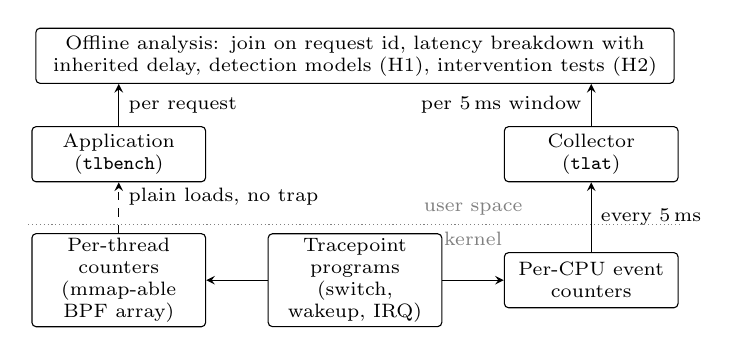
\begin{tikzpicture}[font=\scriptsize, >=stealth,
  box/.style={draw, rounded corners=1.5pt, align=center, inner sep=1.5pt,
              minimum height=0.7cm, text width=2.1cm}]
\node[box] (map)  at (1.2,0)   {Per-thread counters\\(mmap-able BPF array)};
\node[box] (tp)   at (4.2,0)   {Tracepoint programs\\(switch, wakeup, IRQ)};
\node[box] (glob) at (7.2,0)   {Per-CPU event\\counters};
\node[box] (app)  at (1.2,1.6) {Application\\(\texttt{tlbench})};
\node[box] (col)  at (7.2,1.6) {Collector\\(\texttt{tlat})};
\node[box, text width=8.0cm] (ana) at (4.2,2.85)
  {Offline analysis: join on request id, latency breakdown with inherited
   delay, detection models (H1), intervention tests (H2)};
\draw[->] (tp) -- (map);
\draw[->] (tp) -- (glob);
\draw[->, dashed] (map) -- node[pos=0.72, right]{plain loads, no trap} (app);
\draw[->] (glob) -- node[right]{every 5\,ms} (col);
\draw[->] (app) -- node[right]{per request} (app |- ana.south);
\draw[->] (col) -- node[left]{per 5\,ms window} (col |- ana.south);
\draw[gray, densely dotted] (0.05,0.71) -- (8.35,0.71);
\node[gray] at (5.7,0.9) {user space};
\node[gray] at (5.7,0.52) {kernel};
\end{tikzpicture}
\caption{Data path of \sys. Tracepoint programs keep per-thread counters in a
memory-mapped BPF array, which the application reads at request start and
end with no trap; system-wide counters are sampled every 5\,ms as the
aggregate baseline.}
\label{fig:arch}
\end{figure}

\textbf{Validation.} The four time counters come from different
tracepoints, yet for every request they must add up to its service time:
\begin{equation}
t_\mathrm{end}-t_\mathrm{start} = t_\mathrm{oncpu}+t_\mathrm{runq}+t_\mathrm{wake}+t_\mathrm{blocked}.
\label{eq:identity}
\end{equation}

\subsection{Breaking down each request's latency}
A request's latency is split into \emph{sched} (wakeup delay before
service, plus preemption and wakeup waits during service), \emph{irq},
\emph{blocked}, \emph{exec} (on-CPU time minus IRQ time) and \emph{queue}
(time waiting for a free worker). A request can also be late because of an
OS event it never saw: if the request in front of it was preempted, it
waits longer in the queue. We call this \emph{inherited} delay. For request
$i$ and delay type $k \in \{\mathit{sched}, \mathit{irq}, \mathit{blocked}\}$,
\begin{equation}
I_{i,k} = \frac{1}{W} \sum_{j \in C_i} \max\left(0,\; d_{j,k} - 10\,\mu\mathrm{s}\right),
\label{eq:inherited}
\end{equation}
where $C_i$ holds the requests that finished while $i$ waited, $d_{j,k}$ is
their own delay of type $k$, and $W{=}3$ workers; the 10\,$\mu$s floor keeps
many tiny delays from standing in for queue length. The queue time is
then split into inherited sched, irq and blocked parts (capped at the wait)
and a remaining \emph{load} part. A slow request is attributed to the
component that most exceeds the median of the normal requests in the same
run.

\subsection{Detection and attribution analysis}
A request counts as a \emph{tail request} if its latency is above the p99
of separate calibration runs (the median of five runs with seeds
1000--1004, never used for evaluation) for the same workload and load. Each
request has 14 features: 11 counters from its own window and the 3
inherited terms. Times are divided by the tail threshold so that workloads
are comparable, and all features are log-transformed ($\log(1{+}x)$). We
compare a simple rule (total OS delay $>\tau$), logistic regression and a
random forest (150 trees, depth 10), each on three feature sets: the
per-request (\emph{aligned}) features, aggregate counts over 5, 20 or
100\,ms, and a \emph{queue-length control} (the number of requests that
finished during the wait). Models are trained on whole cpu and kv runs
from the main and intervention sets (repetitions 0--2, so stressed runs are
included) and tested on unseen repetitions (3--4) and on the
\textbf{net} workload, which is never used for training or feature design.
Slow requests are rare, so accuracy would be misleading. We report PR-AUC,
the area under the precision--recall curve (a random ranking scores the
fraction of tail requests), with 95\% bootstrap confidence intervals over
runs, plus precision, recall and F1 at the threshold that maximizes F1 on
the training data, and false alarms per minute. To fit in memory we keep
5\% of normal requests and at most 20\,000 tail requests per run, and
weight them back in every metric.

\textbf{Interventions (H2).} At mid load we add one stressor at a time, five
runs each, in random order: a CPU hog on the worker CPUs that runs for 40\%
of every 10\,ms; a softirq flood (UDP over loopback sent from CPU~3, with
Receive Packet Steering (RPS) moving the receive work to CPUs 0--2); an I/O writer (1\,MiB writes
with \texttt{fdatasync}); and an affinity change (a hog on CPU~0 with
workers on CPUs 0--2, compared with workers moved to CPUs 1--2 at 2/3 of
the rate, so that the load per CPU stays the same). Before running them we
wrote down the expected effect of each: hog $\to$ sched, flood $\to$ irq,
I/O $\to$ blocked, moving the workers $\to$ less sched. We then compare the
per-run mean of that delay with the control using a one-sided Mann--Whitney
U test.

\textbf{Reproducibility.} Code, data access and a step-by-step guide with
all tool versions are at
\url{https://github.com/YashvanthSankar/os-course-project};
\texttt{sudo bash scripts/run\_all.sh} reruns all experiments and
regenerates every table and figure.

\section{Experimental Results}
\label{sec:results}
\subsection{Overhead}\label{sec:overhead}
Placeholder.

\FloatBarrier
\section{Conclusion}
\label{sec:conclusion}
\sys{} shows that per-request attribution of OS-induced delay does not
require a trap per request. Per-thread accounting kept by tracepoint
programs and read through a shared BPF map costs about as much as plain
event counters, and its accounting closes. The evaluation gives a more
nuanced answer than our hypothesis. Within a known workload, queueing
explains most tail requests, and any signal that tracks load (including
aggregate counts) detects them. Request-aligned kernel telemetry did
better on one held-out workload, but not when the held-out workload was
rotated or the runs repeated with fresh seeds, so its value lies in naming
the cause, not in detection. Controlled interventions moved
exactly the predicted delay component in seven of nine cases. The
remaining cases, together with the client-side receiver delay of the net
workload, show where the method stops: OS delay on threads outside the
request window, and host effects invisible to the guest. Future work is
to extend windows across all threads a request touches, to model
per-socket queues, and to repeat the study on bare metal. As a by-product,
we prepared a patch that lets bcc's \texttt{runqlat} separate wakeup
latency from preemption latency, the distinction our intervention results
relied on.


\bibliographystyle{IEEEtran}
\bibliography{references}

\end{document}
